% !TEX root = ./pkMain.tex
\mode*
\section{Einleitung}
\mode<all>
% !TEX root = ./pkMain.tex
\mode*


\begin{frame}[<+->]
\mode<presentation>{\frametitle{Einleitung}}
\mode<article>{
	In der An�sthesie dosieren wir die (meisten) Medikamente entsprechend einer gemessenen oder beobachteten Wirkung. Die Zufuhr (Dosis oder Infusionrsate oder Konzentration) wird deshalb w�hrend einer An�sthesie immer wieder angepasst. Dabei kommt die \emph{zeitliche} Dimension des Dosierens ins Spiel. Diese Dimension wird in andern Bereichen der Medizin beim Dosieren weniger explizit ber�cksichtigt:
}
\begin{itemize}
\item
Das klassisches Dosieren (ausserhalb An�sthesie) ist Input basiert $=$ \enquote{Ich lege zum voraus fest, wie gross die Dosis pro KG sein muss?}
\mode<article>{\newline �ber den (exakten) zeitlichen Verlauf der Konzentration resp. Wirkung wird weniger nachgedacht.}
\begin{itemize}
	\item Dosis wird in regelm�ssigen Abst�nden verabreicht (z.B. 1x, 2x pro Tag)
	\item
	Es wird (f�lschlicherweise) angenommen, dass Dosis in eindeutiger Beziehung zur Wirkung steht.
	\item
	Die rechtzeitige Erholung von der Wirkung (\enquote{Aufwachen}) ist nicht wichtig!.
	\item
	Man nimmt an, dass bei gen�gender Dosierung der Therapieerfolg eintritt. Beurteilung des Therapieerfolgs h�ufig \enquote{bin�r} d.h. Erfolg order Nichterfolg
\end{itemize}
\end{itemize}

\mode<article>{
	Die Pharmakokinetik und Pharmakodynamik beschreiben zusammen den Prozess von der Applikation (Aufnahme) des Medikamentes bis zur Wirkung. Dies beinhaltet Aufnahme in Blut (bei oraler Applikation), zeitlicher Verlauf der Konzentration im Blut (Umverteilung, Elimination), zeitlicher Verlauf der Aufnahme und Elimination des Medikamentes in den und aus dem Wirkort sowie die Beziehung zwischen der Konzentration am Wirkort und der Wirkung.
}


\note<1>
{
\begin{itemize}
\item
Wenn ich Gewicht ber�cksichtige nicht mehr weiterdenken?
\\
Beispiel machen: 50 kg x 2 mg Propofol; 100 kg x 2 mg
\item
Was passiert mit dem Medikament nach Injektion, was passiert mit dem Medikament?
\item
Wichtig ist es die Wirkung zu beurteilen\\
Nicht Packungsprospekt = Input; Sondern, was braucht der Patient?
\item
Welche Ziele verfolgen sie? :: Schlaf, evt. schnell Einschlafen, Analgesie, Blutdruck, Herzfrequenz, schmerzfrei Aufwachen, gen�gend Atmen, Reflexe etc.
\end{itemize}
}
\infina
\end{frame}

\begin{frame}[<+->]
\mode<presentation>{\frametitle{Einleitung 2}}

\begin{itemize}

\item
(Klassisches) Dosieren in An�sthesie: Bolus und Infusionsrate
\begin{itemize}
	\item
	Man beginnt evt. mit Bolus (adaptiert gem�ss z.B. Gewicht) oder startet mit einer Infusionrate (wieviel?)
	\item
	Erwartung: Infusionsrate proportional zur Wirkung. (ist nur im SS so!)
	\item
	Situatives dosieren $=$ Anpassen Dosis/Infusionsrate entsprechend der ben\"otigten Wirkung.
	\item
	Auch angepasste Dosis/Infusionsrate NICHT in eindeutiger Beziehung zu Wirkung!
\end{itemize}

\end{itemize}


\note<1>
{
\begin{itemize}
\item
.
\end{itemize}
}
\infina
\end{frame}





\mode<presentation>{
\begin{frame}
	\begin{center}
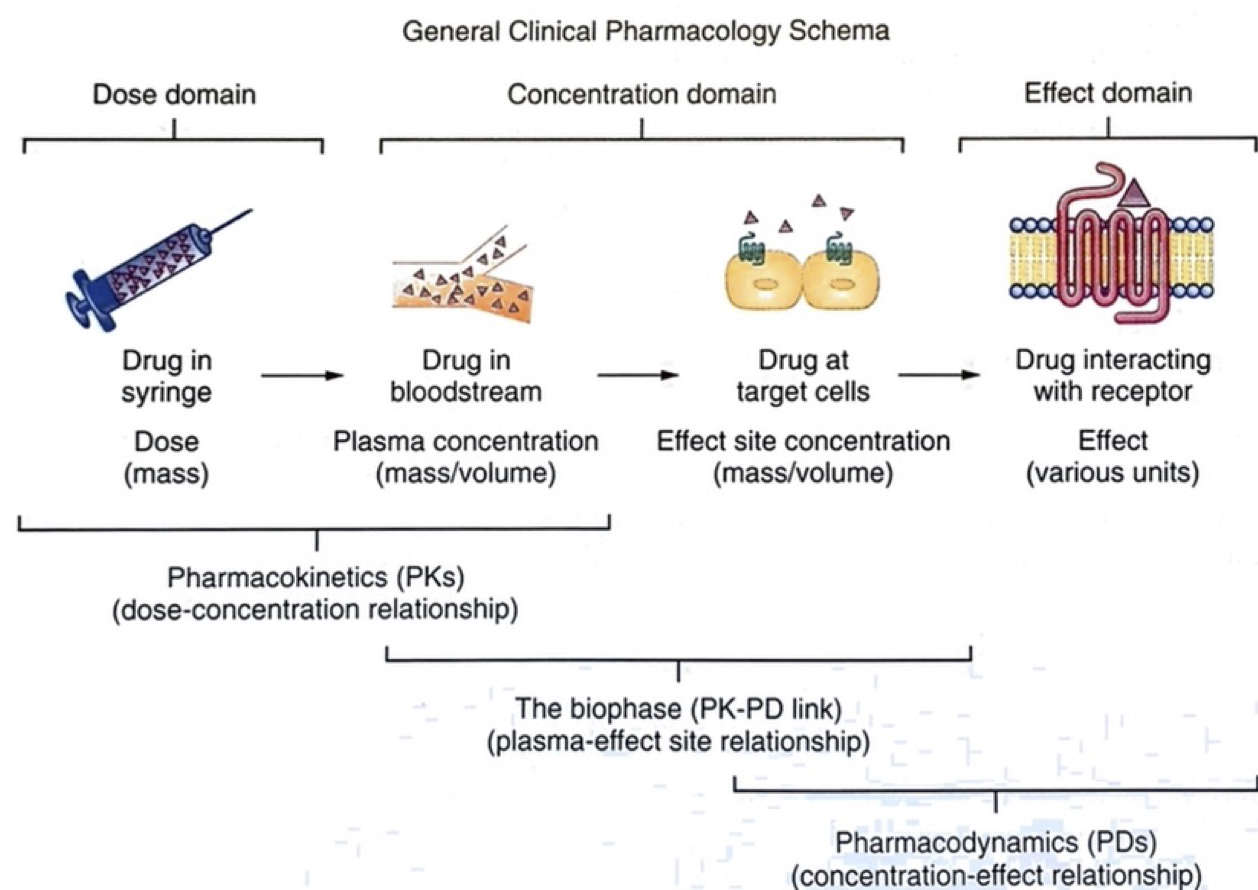
\includegraphics[width=\textheight]{../figures/dose_domains.jpg}
\end{center}
\infina
\end{frame}}

\mode<article>{
\begin{center}
	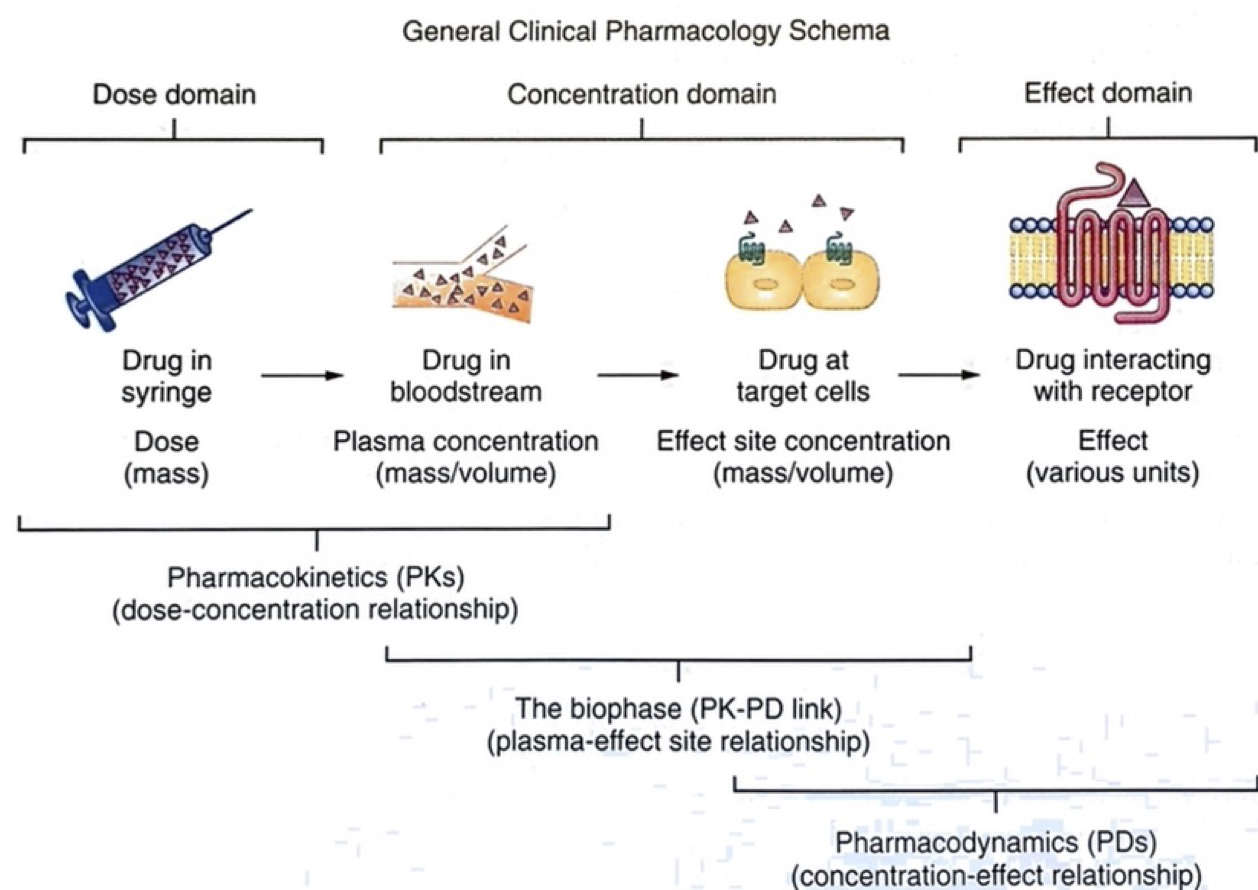
\includegraphics[width=0.6\textwidth]{../figures/dose_domains.jpg}
\end{center}
}


\mode<article>{
	Die Pharmakokinetik und Pharmakodynamik beschreiben zusammen den Prozess von der Applikation (Aufnahme) des Medikamentes bis zur Wirkung. Dies beinhaltet Aufnahme in Blut (bei oraler Applikation), zeitlicher Verlauf der Konzentration im Blut (Umverteilung, Elimination), zeitlicher Verlauf der Aufnahme und Elimination des Medikamentes in den und aus dem Wirkort sowie die Beziehung zwischen der Konzentration am Wirkort und der Wirkung.
}

\section{Grundlagen}
\mode<all>
% !TEX root = ./pkMain.tex
\mode*


\begin{frame}[<+->]
\frametitle{Pharmakokinetik, Pharmakodynamik}
\begin{itemize}
\item
Pharmakokinetik beschreibt was der K�rper mit dem Medikament macht.
\mode<article>{\newline Aufnahme, Verteilung und Elimination des Medikamentes. Beschreibung des zeitlichen Verlaufs der Konzentration.}
\item
Pharmakodynamik beschreibt was das Medikament mit dem K�rper macht
\mode<article>{\newline Beziehung zwischen der (Wirkort-) Konzentration und der Wirkung.}
\end{itemize}

\note<1>{
\begin{itemize}
\item
Beschreiben der zwei S�tze!
\item
Zeichnen: Blut - Organe - Umverteilung - Wirkort - Wirkung
\item
Wenn ein Medikament i.v. verabreicht wird, wird es im Blut verteilt, in verschiedene Organe verteilt und in einigen Organen metabolisiert. Der K�rper \enquote{macht} etwas mit dem Medikament.
\item
Am Wirkort entfaltet das Medikament seine Wirkung (Rezeptor). Das Medikament \enquote{macht} etwas mit dem K�rper.
\item
Cylinder: Kinetik - Input: H�he des zentralen Kompartiments entspricht Konzentration, ist abh�ngig was der K�rper mit dem Input macht.
\end{itemize}
}

\infina
\end{frame}




\mode<all>
% !TEX root = ./pkMain.tex
\mode*


\begin{frame}
\frametitle{Begriffe, Definitionen}
\begin{itemize}
\item<1->
Bolus (Menge, \enquote{Dosis}, z.B. \enquote{\emph{mg}})


\mode<article>{Dosis bezieht sich auf die Menge (Gewicht) der wirksamen Substanz. Achtung die injzierbaren Medikamente sind in einer Fl�ssigkeit gel�st.}
\item
Konzentration: Menge pro Volumen (\enquote{\emph{$\frac{mg}{l}$}})

\mode<article>{Konzentration des Medikamentes im Blut, am Wirkort. Direkte Beziehung zwischen der Konzentration am Wirkort und der Wirkung.}
\item<2->
Infusionsrate (Menge pro Zeit, Infusionsgeschwindigkeit, z.B. \enquote{\emph{$\frac{mg}{h}$}})


\mode<article>{Menge pro Zeit. Die Zeit ist auch bei Bolusgaben zu ber�cksichtigen. Je h�ufiger die Bolusgabe repetiert wird, desto h�her wird die erreichte Konzentration sein. Auch bei repetitiven Bolusgaben wird eine \enquote{Steady State} Konzentration erreicht.}

\end{itemize}
%%%
\note<1>{
\begin{itemize}
\item
Menge in ein Volumen: Substanz verteilt sich homogen $\Rightarrow$ Konzentration. V=10L, 100 mg? 200 mg? - Umgekehrt: 500 mg, Konzentration: 50 mg/ L - Vol?; Zeigen: Nicht homogene Verteilung: sehr grosse VertVol.
Scheinbares Verteilungsvolumen! Rechnerisch!
\item
Hohe Konzentration $=$ hohe Wirkung. (Organ badet im Medikament das im Blut gel�st ist.)
\item
Dosis resp. Infusionsrate $\neq$ Konzentration! (Cylinder: Custom 10 L, IR 10;; 10,30,100 ... dann Fentanyl: IR 2)
\item
Konzentrationsgradient beachten! Nach Stop, in welche Richtung bewegt sich das Medikament?
\end{itemize}
}
\note<2>{
\begin{itemize}
\item
Infusionsgeschwindigkeit: Volumen pro Zeit, Verd\"unnung des Medikamentes, weil Menge pro Zeit wichtig ist.\\
Sie geben 2\% Propofol mit Rate 6mg/kg/h -nach dem Wechsel auf 1\% Propofol wieviel m�ssen sie geben?
\item
Bolus: Je nach zeitl. Beziehung andere Konzentration - Wirkung
\end{itemize}
}
%%%
\infina
\end{frame}


\section{Therapieziel Wirkung}
\mode<all>
% !TEX root = ./pkMain.tex
\mode*

\begin{frame}
\frametitle{Was sollten wir am \enquote{Infusionsger\"at} einstellen?}
\begin{itemize}[<+->]
\item
Die Wirkung korreliert mit der \emph{Konzentration am Wirkort}.\\
\mode<article>{Bei normalen Spritzenpumpen kann aber nur die Infusionsrate eingestellt werden!.}
\item
Je mehr Medikament am Wirkort, desto h�her die Konzentration. 
\item
Mit einem Verdampfer f�r volatile An\"asthetika werden Konzentrationen eingestellt! 
\end{itemize}

\note<1>{
\begin{itemize}
\item
An Verdampfer stellen wir eine Konzentration ein
\item
Bei i.v. An\"asthesie
\item
Simulation konstante Infusion Alfentanil:\\
15 min IR: 50 $\Rightarrow$ Konz.: 64\\
bis 30 min. IR: 100 $\Rightarrow$ Conc.: 92.5
dann wieder 50 $\Rightarrow$ KonZentration steigt eher an!
\end{itemize}
}
\infina
\end{frame}


\mode<all>
% !TEX root = ./pkMain.tex
\mode*


\frame{
\mode<presentation>{
\begin{tikzpicture}[remember picture, overlay]
\node[inner sep=0pt,xshift=0cm] at (current page.center){
\tikz \draw[step=2mm,black!50] (0,0) grid (126mm,94mm);
};
{
\node[coordinate] at (1cm,-3.55cm) (start) {};
\node[coordinate] at (1cm,3cm) (end) {};
\node[coordinate] at (10cm,-3.55cm) (endy) {};
\draw[->,thick] (start)--(end);
\draw[->,thick] (start)--(endy);
};
\end{tikzpicture}
}
\frametitle{Konzentration am Wirkort $\Rightarrow$ Wirkung}

\note<1>{
\begin{itemize}
\item
Rezeptoren - endliche Zahl
\item
H\"ohere Konzentration: Keine zus\"atzliche Wirkung
\item
Begriff der Potenz: $\neq$ St\"arke: Bedeutung - Zusammenhang zu Sensitivit\"at
\item
Therapeutische Fenster
\item
Vorstellung haben  wie die Kurve bei einem Patienten verl\"auft. Steilheit absch\"atzen.
\item
Verstehen warum aufwachen so unterschiedlich sein kann
\end{itemize}
}
\infina
}

\mode<article>{
\vspace{1cm}
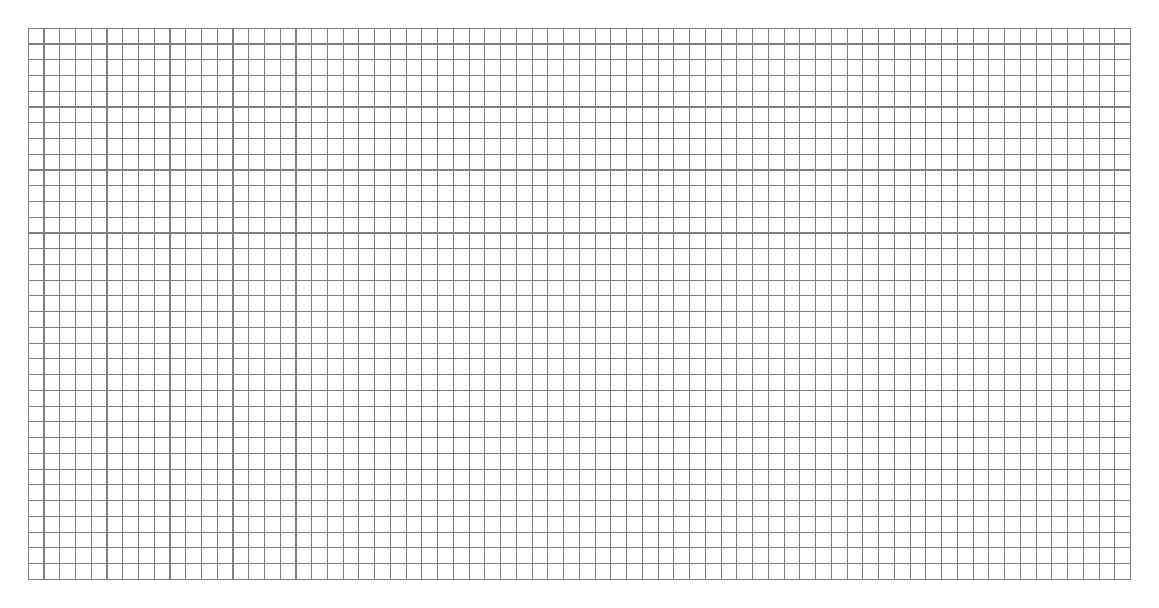
\begin{tikzpicture}[auto]
\node[inner sep=0pt,xshift=0cm] at (current page.center){
\tikz \draw[step=2mm,black!50] (0,0) grid (140mm,70mm);
};
\end{tikzpicture}
}


\mode<article>{\pagebreak}
\section{Input Beziehung zur Konzentration}
\mode<all>
% !TEX root = ./pkBeamer.tex
\mode*

\frame{
\mode<presentation>{
\begin{tikzpicture}[remember picture, overlay]
\node[inner sep=0pt,xshift=0cm] at (current page.center){
\tikz \draw[step=2mm,black!50] (0,0) grid (126mm,94mm);
};
{
\node[coordinate] at (1cm,-3.55cm) (start) {};
\node[coordinate] at (1cm,3cm) (end) {};
\node[coordinate] at (10cm,-3.55cm) (endy) {};
\draw[->,thick] (start)--(end);
\draw[->,thick] (start)--(endy);
};
\end{tikzpicture}
}
\frametitle{Bolus: Fixe \enquote{Menge}}



\note<1>{
\begin{itemize}
\item
Zeichnen: 1 Kompartiment, Injektion, dann mit Cylinders.
\item
Konzentration f\"allt in jedem Intervall auf die H\"alfte ab
\item
Zeichenn Abfall �ber Zeit
\end{itemize}
}
\infina
}


\mode<article>{
\vspace{1cm}
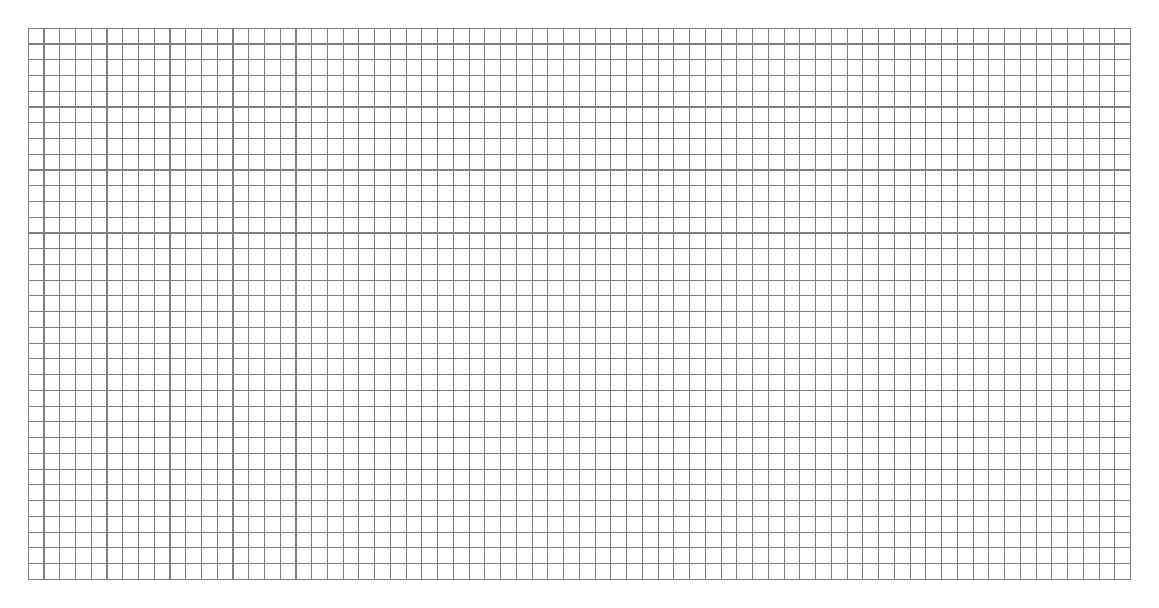
\begin{tikzpicture}[auto]
\node[inner sep=0pt,xshift=0cm] at (current page.center){
\tikz \draw[step=2mm,black!50] (0,0) grid (140mm,70mm);
};
\end{tikzpicture}
}

\mode<article>{\vspace{1cm}
	Unmittelbar nach i.v. Injektion ist die Konzentration im Blut am h�chsten. (theoretisch: $\frac{Dosis}{Blutvolumen}$). Im Gehirn resp. im Gewebe ist aber noch kein Medikament angekommen. Wirkeintritt ist verz�gert gegen�ber Verlauf der Blutkonzentration.

	Konzentration im Blut f�llt exponentiell ab. Geschwindigkeit des Konzentrationsabfalls ist abh�ngig vom Medikament.


}


\frame{
\mode<presentation>{
\begin{tikzpicture}[remember picture, overlay]
\node[inner sep=0pt,xshift=0cm] at (current page.center){
\tikz \draw[step=2mm,black!50] (0,0) grid (126mm,94mm);
};
{
\node[coordinate] at (1cm,-3.55cm) (start) {};
\node[coordinate] at (1cm,3cm) (end) {};
\node[coordinate] at (10cm,-3.55cm) (endy) {};
\draw[->,thick] (start)--(end);
\draw[->,thick] (start)--(endy);
};
\end{tikzpicture}
}

\mode<article>{\newpage}

\frametitle{Konstante Infusion: Konstante (fixe) \enquote{Rate}}
\note<1>{
\begin{itemize}
\item
Zeichnen: Minuten Intervall: Jede Minute wird eine bestimmte Menge verabreicht. 100 mg/min in 10 L
\item
Konzentration w\"urde einfach ansteigen, wenn keine Elimination.
\item
Simulation mit Cylinder 1 Kompartiment (Cl = 0)
\item
Mit Elimination
\item
Auf X-y zeigen wie das passiert. (Behandelt eigentlich schon Elimination)
\end{itemize}
}
\infina
}

\mode<article>{
\vspace{1cm}
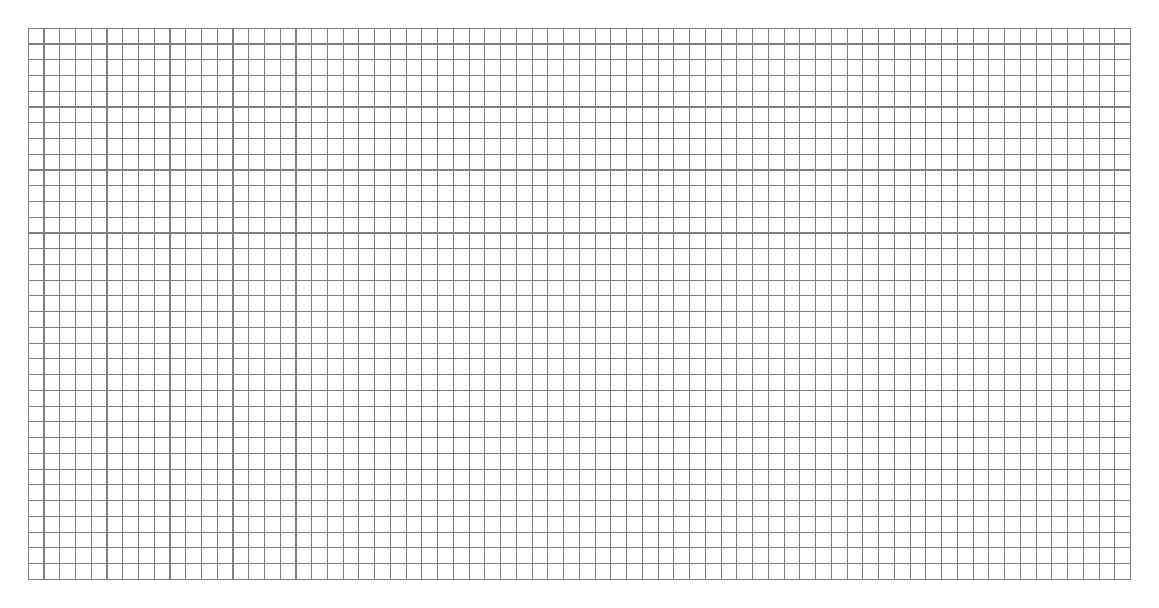
\begin{tikzpicture}[auto]
\node[inner sep=0pt,xshift=0cm] at (current page.center){
\tikz \draw[step=2mm,black!50] (0,0) grid (140mm,70mm);
};
\end{tikzpicture}

\vspace{0.5cm}


Eine konstante Zufuhr(rate) hat nicht einfach eine konstante Konzentration zur Folge. Die Zufuhr muss im Zusammenhang mit der Elimination betrachtet werden (siehe Elimination!) Da die Elimination(srate) proportional zur Konzentration ist, steigt die Konzentration bei konstanter Zufuhr initial an.


Wie lange steigt die Konzentration an?
}





\begin{frame}
\note<1>{
Es ist etwas Komplexer!\\
Kompartimente zeichnen.\\
Zeigen, dass Medi in zentrale Kompartiment verabreicht werden\\
Zeigen der Verteilung\\
Weglassen der Umverteilung\\
Annahme, dass Elimination proportional zu Konzentration.\\
Cylinder: Propofol - IR: Erkl�ren der Dicke der Pfeile = Menge.

}
\end{frame}




\section{Elimination, Umverteilung}
\mode<all>
% !TEX root = ./pkMain.tex
\mode*

{Die Medikamenten Konzentration im Blut f�llt ab, weil das Medikament (aus dem K�rper) eliminiert, metabolisiert und umverteilt wird. {\it{Elimination}} kann aber im pharmakokinetischen Sinne auch allgemein den \enquote{Abfall} der Konzentration beschreiben. Es gibt verschiedene Begriffe mit denen die Elimination quantifiziert wird: Halbwertszeit, Clearance, Eliminationsrate. Keiner dieser Begriffe beschreibt alleine gen�gend ob die Konzentration in einer gegeben Situation schnell oder langsam abf�llt. Ein sehr wichtiger, die Elimination beschreibender Prozess ist die {\it{Clearance}}. Die {\it{Kontext sensitiven Konzentrationsabfallzeiten}} (siehe weiter hinten) beschreiben den Konzentrationsabfall resp. die Elimination umfassend.

\begin{frame}
\frametitle{Elimination, Grunds\"atzliches}
\begin{itemize}[<+->]
\item
Eliminationsrate $=$ Menge die pro Zeit eliminiert wird
\item
Eliminationsrate abh\"angig von der Konzentration


\mode<article>{Dies gilt f�r (alle) An�sthetika. Im Rahmen von klinisch \enquote{sinnvollen} Konzentrationen ist die Kapazit�t der Eliminationsprozesse nicht ausgesch�pft. Deshalb wird mehr eliminiert, wenn die Konzentration h�her ist. Man spricht in diesem Falle von {\it linearer} Kinetik. 

Es gibt auch {\it nicht lineare} Kinetik! Wie w�rde die Konzentration bei \emph{nicht linearer} Kinetik (Eliminationsrate unabh�ngig von Konzentration!) abfallen? Beispiel?}
\item
Achtung: Die {\it Zufuhrrate} ist mit einer konstanten Infusion konstant! Bei linearer Kinetik ist die Elimination aber abh�ngig von der Konzentration!
\end{itemize}
\note<1>{
\begin{itemize}
\item
...
\end{itemize}
}
\infina
\end{frame}




\begin{frame}
\frametitle{Clearance: Volumen pro Zeit, z.B. $\frac{ml}{min}$}
\begin{itemize}[<+->]
\item
Beschreibt Volumen das pro Zeit \enquote{gereinigt} wird.
\item
Proportionalit�tskonstante: Eliminationsrate in Beziehung zu Konzentration.
\item
Wenn Konzentration hoch: Eliminationsrate hoch
\item
Wie hoch kann bei einer konstanten Zufuhr (Infusionsrate) die Elimininationsrate maximal werden? (Zufuhr und Elimination finden gleichseitig statt.)
\end{itemize}

\note<1>{
\begin{itemize}
\item
Quadrat mit 3 er Unterteilung
\item
Jedes Teilvolumen 1 l, Totalvolumen $=$ 9 l
\item
Clearance ist 1l / min
\item
Wie lange geht es bis das ganze Volumen gereinigt.
\item
Simulation mit Cylinder: Dicke der Pfeile zeigen.
\end{itemize}
}
\infina
\end{frame}

\mode<article>{\pagebreak}
\section{Input und Elimination}
\mode<all>
% !TEX root = ./pkMain.tex
\mode*

\begin{frame}
\frametitle{Steady State Konzentration}
\begin{itemize}[<+->]
\item
Abh�ngig von Infusionsrate und ?
\item
Warum geben wir Katecholamine nicht mit TCI?
\end{itemize}
\note<1>{
Rise2SS.xls}
\infina
\end{frame}


\begin{frame}
\begin{itemize}[<+->]
\item
Propofol wird mit 6 mg/kg/h einem 70 Kilo Patienten infundiert.
\item
Was m�ssen sie wissen, damit sie berechnen k�nnen wie hoch die Konzentration ist?
\end{itemize}
\note<1>{
$C_{ss}=\frac{R}{Cl}$\\
Clearance ist eingeschr�nkt?\\
}
\end{frame} 
\mode<all>
% !TEX root = ./pkMain.tex
\mode*

\begin{frame}
\frametitle{Verteilungsvolumen}
\begin{itemize}[<+->]
\item
Summe der Volumina
\item
Auch Proportionalit�tskonstante! (Menge von Medikament im K�rper und Konzentration)
\end{itemize}
\note<1>{
\begin{itemize}
\item
Summe der Volumina
\item
Kann sehr gross werden, wenn Medikament in Gewebe angereichert.
\end{itemize}
}
\infina
\end{frame}


Um die Eliminationsgeschwindigkeit zu beurteilen, m�ssen {\it Verteilungsvolumen} und die {\it Clearance} zusammen betrachtet werden. Der initiale Konzentrationsabfall ist aber eine Folge der Umverteilung des Medikamentes (aus dem Blut) und die Gr�sse des Verteilungsvolumens spielt eine dabei eine Rolle.
\mode<article>{\pagebreak}





